%% RAMT paper draft for Engineering Applications of Artificial Intelligence (Elsevier).
%% Compile on Overleaf with pdfLaTeX + BibTeX (Overleaf does this automatically).
%% Red text marks items still to be filled in (pending runs, EAAI citations, author data).
\documentclass[preprint,12pt,authoryear]{elsarticle}

\usepackage{amsmath,amssymb}
\usepackage{graphicx}
\usepackage{booktabs}
\usepackage{multirow}
\usepackage{xcolor}
\usepackage{hyperref}
\usepackage{siunitx}
\sisetup{group-separator={,},group-minimum-digits=4}

\newcommand{\pending}[1]{\textcolor{red}{[#1]}}
\newcommand{\todo}[1]{\textcolor{red}{[TODO: #1]}}

\journal{Engineering Applications of Artificial Intelligence}

\begin{document}

\begin{frontmatter}

\title{Rationale-supervised attention for multi-task hate-speech detection: human-aligned, faithful explanations at no accuracy or latency cost}

\author[inst1]{Veena Shanmukh Bagildavar}
\ead{veenashanmukhbagildavarbtech24@rvu.edu.in}
\author[inst1]{Varsha Shivanand K}
\ead{varshashivanandkbtech24@rvu.edu.in}
\author[inst1]{Yashwitha T S}
\ead{yashwithatsbtech24@rvu.edu.in}
\author[inst1]{Madderla Chiranjeevi\corref{cor1}}
\ead{madderlachiranjeevi@rvu.edu.in}
\cortext[cor1]{Corresponding author.}
\affiliation[inst1]{organization={School of Computer Science and Engineering, RV University},
            city={Bengaluru},
            country={India}}

\begin{abstract}
Content moderation systems must flag explicit abuse, implicit hate and offensive language, and moderators need to see \emph{why} a post was flagged. Post-hoc explainers such as Integrated Gradients (IG) and LIME add latency, and attention weights are often neither faithful nor human-like. We present RAMT, a multi-task RoBERTa model with one attention pool per task, in which the hate-speech head's attention is trained to match human word-level rationales from HateXplain. Against two controls that share data, encoder, schedule and seeds (no rationale loss, and the same rationale signal placed on random words), human rationales raised attention plausibility from 0.69 and 0.40 to 0.92 token-AUPRC and attention faithfulness (AOPC comprehensiveness above random) from 0.28 and 0.01 to 0.46. All four effects were confirmed in a family of 12 tests, specified before any test-set evaluation,  that combine seed and test-sampling uncertainty under Holm correction, and all five seeds agreed. Classification was unchanged on Jigsaw, the Implicit Hate Corpus and HateXplain (all differences $\le 0.003$). The effect transferred to the explicit-toxicity head, which never sees rationales (plausibility 0.89 vs.\ at most 0.55). The attention explanation was as faithful as IG within a validation-derived margin and added no latency (15\,ms per post on a T4 GPU), where IG took 4.8$\times$ and LIME 22.8$\times$ as long; on a 4-thread CPU the factors were 52$\times$ and 281$\times$. Multi-task training did not improve over single-task models, and the GPU speed target set in advance (IG at least 10$\times$ slower) was not met.
\end{abstract}

%% Highlights (Elsevier: 3-5 bullets, max 85 characters each)
\begin{highlights}
\item Human rationales make a detector's own attention a usable explanation.
\item A random-rationale control shows the gain comes from the human rationales.
\item Rationale-trained attention also transfers to a head trained without them.
\item Attention matches Integrated Gradients' faithfulness at no extra latency.
\item Accuracy is unchanged; a small, non-significant bias gap is reported.
\end{highlights}

\begin{keyword}
hate speech detection \sep explainable artificial intelligence \sep rationale supervision \sep attention \sep multi-task learning \sep faithfulness \sep content moderation
\end{keyword}

\end{frontmatter}

%% ===================================================================
\section{Introduction}
\label{sec:intro}

Online platforms rely on automated classifiers to triage abusive content at a scale no human team can review. Abuse takes more than one form, though. Explicit toxicity (insults, threats, obscenity) is lexically marked. Implicit hate is carried by stereotypes, irony or coded language and usually contains no slur \citep{elsherief2021latent}. A third group of posts is offensive without being hateful \citep{mathew2021hatexplain,zampieri2019olid}. A moderator who reviews a flagged post also needs to know \emph{which words} drove the decision, both to act quickly and to catch the model when it is wrong. In this application explainability is an operational requirement, not an add-on.

Two families of explanation are common. Post-hoc attribution methods such as Integrated Gradients (IG) \citep{sundararajan2017axiomatic} and LIME \citep{ribeiro2016lime} work with any model but need many extra forward or backward passes per post, which adds latency in a moderation queue. Attention weights come free with the prediction, but whether they explain anything is disputed \citep{jain2019attention,wiegreffe2019attention}: unsupervised attention is often neither \emph{plausible} (it does not match what humans point to) nor \emph{faithful} (removing the highly weighted words changes the prediction little) \citep{jacovi2020faithfully,deyoung2020eraser}. HateXplain \citep{mathew2021hatexplain} supplies human word-level rationales for hateful and offensive posts and showed that supervising attention with them can raise plausibility. It trained a single-task model, however, did not compare the gain with a control that receives the same amount of extra supervision on random words, and did not measure cost against post-hoc explainers.

This paper asks whether rationale supervision can make a model's own attention a usable explanation inside a multi-task detector, at no cost in accuracy or speed. We make four contributions:
\begin{enumerate}
\item \textbf{RAMT}, a multi-task model on a shared RoBERTa encoder \citep{liu2019roberta} with one additive attention pool per task (explicit toxicity, implicit hate, and hate/offensive/normal). Only the HateXplain head's attention receives the rationale-alignment loss.
\item \textbf{A controlled test of rationale supervision.} Two controls share every other setting with RAMT: one has no rationale loss, the other receives the same loss on random words matched in number and mass to the human rationale. This separates the effect of \emph{human} rationales from that of extra supervision as such. Hypotheses, metrics, margins and the 12-test confirmatory family were fixed before any test-set result was seen, and the tests combine seed and test-sampling variance under Holm correction.
\item \textbf{Evidence of transfer.} We test whether attention trained to match rationales on one head becomes more plausible on heads that never see rationales.
\item \textbf{A cost comparison} of attention against IG and LIME on the same fixed post sets, covering faithfulness and per-post latency.
\end{enumerate}

The results are mixed in an informative way. Human rationales made the attention both more plausible and more faithful, beyond the random-rationale control, and the gain transferred to the explicit-toxicity head. Attention matched IG's faithfulness within a margin fixed in advance while adding no latency. Multi-task training, however, did not beat single-task models, the speed targets set in advance against IG and LIME were met on CPU but not on GPU, and rationale-trained models scored lower on a subgroup-bias metric (the difference was not significant). Section~\ref{sec:related} reviews related work, Section~\ref{sec:method} describes RAMT, Section~\ref{sec:setup} the experimental protocol, Section~\ref{sec:results} the results and Section~\ref{sec:discussion} their limits.

%% ===================================================================
\section{Related work}
\label{sec:related}

\paragraph{Hate-speech and toxicity detection}
Automatic detection of abusive language has moved from lexicon and feature-based classifiers to fine-tuned transformer encoders \citep{fortuna2018survey,mishra2024shielding}. \citet{davidson2017automated} showed early that hateful and merely offensive language are easily confused, which motivates three-way label schemes such as HateXplain's \citep{mathew2021hatexplain}. Domain-adapted encoders such as HateBERT \citep{caselli2021hatebert} are further pre-trained on abusive text, while general encoders such as BERT \citep{devlin2019bert}, RoBERTa \citep{liu2019roberta} and DeBERTa \citep{he2021deberta} remain strong baselines. Recent work in this journal has extended detection to multimodal posts \citep{chhabra2023multimodal}, to English and German text with optimised feature extraction \citep{kar2023sentimental}, to multilingual offensive-language filtering \citep{saumya2024filtering}, to cross-lingual transfer with contrastive and adversarial learning \citep{almahdi2025crosslingual}, and to transformer ensembles for lower-resource languages \citep{aksoy2026turkish}. Benchmarks cover different forms of abuse: Jigsaw toxic comments (multi-label explicit toxicity) \citep{jigsaw2018toxic}, OLID \citep{zampieri2019olid}, the Implicit Hate Corpus \citep{elsherief2021latent}, ToxiGen \citep{hartvigsen2022toxigen} and HateXplain. The quality and label definitions of these datasets vary widely \citep{vidgen2020directions}, and functional tests such as HateCheck \citep{rottger2021hatecheck} expose systematic false positives on non-hateful posts that mention identity groups.

\paragraph{Large language models}
Prompted large language models (LLMs) can classify hateful content and produce free-text explanations \citep{huang2023chatgpt,roy2023probing}, and their role in moderation pipelines is now widely discussed \citep{ahmad2026detection}. Their outputs are sensitive to prompt wording and to sensitive terms in otherwise benign posts \citep{roy2023probing}, and a generated explanation is not guaranteed to reflect the computation behind the label. They also cost far more per post than an encoder. We therefore study explanations that come from the classifier's own computation at encoder cost, and leave comparison with LLM explanations to future work.

\paragraph{Multi-task learning for abuse detection}
Sharing an encoder across related tasks is meant to transfer signal between datasets with different label schemes \citep{ruder2017overview}. In abuse detection, \citet{kapil2020deep} combined several hate-speech datasets in a shared deep network, and \citet{zampieri2023offensive} reported gains from predicting offensiveness at post and token level jointly. Gains are not guaranteed, however, and depend on how closely tasks are related and how batches are sampled. We sample tasks in proportion to the square root of their training-set size and test multi-task against single-task training directly (H1).

\paragraph{Attention as explanation}
\citet{jain2019attention} and \citet{serrano2019attention} showed that attention weights often disagree with gradient-based importance and can be altered without changing predictions; \citet{wiegreffe2019attention} argued that this does not rule attention out as an explanation in every setting. \citet{jacovi2020faithfully} separated plausibility (agreement with humans) from faithfulness (agreement with the model's own reasoning), and the ERASER benchmark \citep{deyoung2020eraser} made both measurable, through token-level overlap with human rationales and through comprehensiveness and sufficiency under word removal. \citet{atanasova2020diagnostic} compared gradient, perturbation and simplification-based explainers on such criteria and found no method best on all of them. We use ERASER's area-over-the-perturbation-curve (AOPC) form, corrected for a random-removal baseline.

\paragraph{Supervising models with human rationales}
Using annotator rationales as extra supervision goes back to \citet{zaidan2007using} and was carried into neural text classifiers by \citet{zhang2016rationale}. For hate speech, \citet{mathew2021hatexplain} added an attention-supervision loss on HateXplain rationales and reported better plausibility at similar accuracy, and \citet{kim2022hate} used masked rationale prediction as an intermediate task to improve both explanations and bias metrics. \citet{kennedy2020contextualizing} took the converse route and regularised post-hoc explanations so that classifiers rely less on group identifiers. None of these studies compared human rationales with a control that receives the same amount of supervision on random words, so they could not separate the effect of \emph{human} rationales from that of any extra constraint on attention. Our random-matched control (M3) does this.

\paragraph{Post-hoc explainers and their cost}
IG \citep{sundararajan2017axiomatic} integrates gradients along a path from a baseline input and satisfies completeness in the limit of many steps; LIME \citep{ribeiro2016lime} and SHAP \citep{lundberg2017unified} fit local surrogate models to many perturbed copies of the input. All need many extra forward or backward passes. Few studies of hate-speech detection report explanation latency alongside faithfulness, although latency decides whether an explanation can be shown in a live moderation tool; responsible moderation systems increasingly treat transparency as a design requirement \citep{asante2026responsible}.

\paragraph{Fairness in toxicity classifiers}
Identity terms and dialect can drive false positives \citep{dixon2018measuring,sap2019risk}. \citet{borkan2019nuanced} introduced subgroup AUC metrics (Subgroup, BPSN, BNSP), and HateXplain aggregates them over target communities with a generalised mean. Explainable methods have also been proposed to locate bias in text directly \citep{kurup2026explainable}. We report the BPSN component as a guard-rail test (F).

%% ===================================================================
\section{Method}
\label{sec:method}

\subsection{Architecture}
A post is split into words, truncated to $W=159$ words, and tokenised into at most $L=232$ sub-words (both limits cover the long tail of the training data; $L$ was fixed by a GPU benchmark before training). A RoBERTa-base encoder produces hidden states $h_j \in \mathbb{R}^{768}$. Each task $t$ has its own additive attention pool over the \emph{content} sub-words (padding and special tokens excluded):
\begin{equation}
s^{t}_{j} = v_t^{\top}\tanh\!\left(W_t h_j + b_t\right), \qquad
\alpha^{t}_{j} = \frac{\exp s^{t}_{j}}{\sum_{k \in \mathcal{C}} \exp s^{t}_{k}}, \qquad
z^{t} = \sum_{j \in \mathcal{C}} \alpha^{t}_{j} h_j ,
\end{equation}
with $W_t \in \mathbb{R}^{256\times768}$ and $\mathcal{C}$ the content positions. A linear head maps $z^{t}$ (after dropout 0.1) to the task outputs: six sigmoid outputs for Jigsaw (\textit{toxic, severe toxic, obscene, threat, insult, identity hate}), one sigmoid output for IHC (implicit hate vs.\ not hate), and a three-way softmax for HateXplain (hate, offensive, normal). Scores and the softmax are computed in fp32. The attention vector $\alpha^{t}$ of each head is the explanation that head gives; word scores are obtained by summing $\alpha^{t}$ over each word's sub-words.

\subsection{Task losses}
The Jigsaw and IHC heads use binary cross-entropy with positive-class weights $w_k=\mathrm{clip}\big(\sqrt{n^{-}_k/n^{+}_k},\,1,\,10\big)$ computed from training counts; the HateXplain head uses cross-entropy.

\subsection{Rationale-alignment loss}
In HateXplain each post was labelled by three annotators, and annotators who called a post hateful or offensive marked the words that justify their label. Let $r^{(a)}\in\{0,1\}^{n}$ be annotator $a$'s rationale vector over the post's $n$ words. The soft word-level target is the mean over the annotators who supplied one, $\rho_i = \frac{1}{|A|}\sum_{a\in A} r^{(a)}_i$. Each word's mass is split evenly over its sub-words, giving $q_j$, which is normalised to $\tilde q_j = q_j/\sum_k q_k$. For a batch of $B$ HateXplain posts the loss is the cross-entropy between the target and the HateXplain head's attention,
\begin{equation}
\mathcal{L}_{\text{rat}} = \frac{1}{B}\sum_{p \in \mathcal{E}} \Big(-\sum_{j} \tilde q_{p,j}\,\log\big(\alpha^{\text{hx}}_{p,j}+\epsilon\big)\Big),
\end{equation}
where $\mathcal{E}$ is the set of \emph{eligible} posts in the batch (majority label hate or offensive, at least one rationale, non-empty target after truncation) and $\epsilon=10^{-8}$. Dividing by $B$ rather than $|\mathcal{E}|$ gives each eligible post the same weight and makes the loss exactly zero when no post is eligible. On a HateXplain batch the total loss is $\mathcal{L}_{\text{hx}} + \mu\,\mathcal{L}_{\text{rat}}$ with $\mu=1$; Jigsaw and IHC batches use their task loss alone. Neither the Jigsaw nor the IHC head ever receives rationale supervision.

\subsection{Random-matched control}
To separate the effect of \emph{human} rationales from that of any extra constraint on attention, the control model M3 receives the same loss with the same weight, but on a target in which each post's own $\rho$ values are permuted to random word positions (one fixed permutation per post). The target therefore has the same number of marked words and the same mass distribution as the human target, but on the wrong words.

\subsection{Multi-task training}
Training runs in rounds of 1{,}000 optimisation steps. Each step draws one single-task batch of 32 posts; the number of steps per task in a round is proportional to the square root of that task's training-set size (temperature 2), and the order of steps within a round is shuffled. Posts are bucketed by length. We train for six rounds with AdamW (learning rate $2\times10^{-5}$, weight decay 0.01, 6\% linear warm-up then linear decay, gradient clipping at 1.0) and mixed precision (fp16 autocast with fp32 master weights). After each round the model is scored on the validation sets (Jigsaw macro-AUPRC, IHC AUPRC, HateXplain macro-F1 with arg-max predictions), and the round with the best mean score is kept. Decision thresholds for the binary outputs are then set on validation by maximising F1 averaged over 200 bootstrap resamples, and temperatures are fitted on validation. The test sets are used only once, for the final evaluation.

%% ===================================================================
\section{Experimental setup}
\label{sec:setup}

\subsection{Data}
Table~\ref{tab:data} summarises the data. \textbf{Jigsaw} toxic comments \citep{jigsaw2018toxic} (explicit toxicity, six labels): the validation set (\num{15901} comments) is held out from the official training file; the training set keeps every remaining toxic comment and a random sample of \num{30000} of the \num{129011} clean ones, giving \num{44306} comments after de-duplication; the test set is the \num{63978} official test comments that carry labels. \textbf{IHC} stage-1 posts \citep{elsherief2021latent}: implicit hate vs.\ not hate, split into \num{14254}/\num{2039}/\num{4079} posts; the \num{1089} explicit-hate posts are kept out of training and used only as a probe. \textbf{HateXplain} \citep{mathew2021hatexplain}: the official train/validation/test division, \num{15318}/\num{1920}/\num{1924} posts after removing cross-split near-duplicates from train and validation (the official test set is untouched); posts without a majority label are excluded, and 59.4\% of posts in each split are eligible for the rationale loss. \textbf{HateCheck} \citep{rottger2021hatecheck} (\num{3728} functional test cases, 29 functionalities) is used only for evaluation. Inputs are truncated to $W=159$ words; the 95th percentile of post length is 217 words for Jigsaw, 49 for HateXplain and 29 for IHC.

\begin{table}[t]
\centering
\caption{Datasets after preparation. Positive rate: share of posts with at least one toxicity label (Jigsaw), labelled implicit hate (IHC), or labelled hate or offensive (HateXplain).}
\label{tab:data}
\small
\resizebox{\textwidth}{!}{\begin{tabular}{llrrrr}
\toprule
Dataset & Task & Train & Validation & Test & Positive rate (train / test) \\
\midrule
Jigsaw & explicit toxicity, 6 labels & \num{44306} & \num{15901} & \num{63978} & 32.7\% / 9.8\% \\
IHC & implicit hate vs.\ not hate & \num{14254} & \num{2039} & \num{4079} & 34.8\% / 34.8\% \\
HateXplain & hate / offensive / normal & \num{15318} & \num{1920} & \num{1924} & 59.4\% / 59.4\% \\
HateCheck & functional tests (evaluation only) & -- & -- & \num{3728} & -- / 68.8\% hateful \\
\bottomrule
\end{tabular}}
\end{table}

\subsection{Models}
Table~\ref{tab:models} lists the models. M1--M3 form the core comparison and differ only in the rationale target. M4 and M4b share one attention pool across tasks (with and without rationale loss), M5 and M6 are single-task models, M7 are task pairs, M8 swap the encoder, and CLS models classify from the \texttt{[CLS]} token instead of an attention pool. M1--M3 were trained with five seeds (42, 123, 2024, 7, 999), the others with three (42, 123, 2024). Encoder, learning rate, $\mu$ and the rationale aggregation were chosen in a pilot with a separate seed on validation data only (Section~\ref{sec:pilot}).

\begin{table}[t]
\centering
\caption{Models compared. All use RoBERTa-base unless stated.}
\label{tab:models}
\small
\resizebox{\textwidth}{!}{\begin{tabular}{lll}
\toprule
Model & Tasks & Description \\
\midrule
M1 RAMT & Jigsaw, IHC, HX & per-task attention pools; human-rationale loss on HX head ($\mu=1$) \\
M2 & Jigsaw, IHC, HX & as M1, no rationale loss ($\mu=0$) \\
M3 & Jigsaw, IHC, HX & as M1, rationale loss on random-matched target \\
M4 / M4b & Jigsaw, IHC, HX & one shared attention pool; with / without rationale loss \\
M5 & one task & single-task, no rationale loss \\
M6 & HX & single-task with human-rationale loss \\
M7 & two tasks & task pairs, no rationale loss \\
M8 & Jigsaw, IHC, HX & as M2 with HateBERT or DeBERTa-v3-base \\
CLS & one task & single-task, \texttt{[CLS]} pooling \\
\bottomrule
\end{tabular}}
\end{table}

\subsection{Metrics}
\paragraph{Classification} Jigsaw macro-AUPRC over the six labels, IHC AUPRC, and HateXplain macro-F1 are the primary metrics. We also report tuned-threshold F1 scores.

\paragraph{Plausibility} Token-level AUPRC between a head's word scores and the majority gold rationale (words marked by at least half of the annotators), averaged over the HateXplain test posts with a hate or offensive majority. Random word scores give 0.381 on this set. For the explicit and implicit heads (hypothesis H3) the same measure is applied to those heads' attention on the same HateXplain posts.

\paragraph{Faithfulness} AOPC comprehensiveness \citep{deyoung2020eraser}: the mean drop in the predicted-class probability when the top 1, 5, 10, 20 and 50\% of words by explanation score are deleted, minus the same quantity for random deletion (five random draws). Sufficiency is computed analogously by keeping only those words (lower is better). To make comparisons paired, all models and explanation methods are scored on one fixed set per test set: up to \num{1000} gold-positive posts drawn once with a fixed seed.

\paragraph{Explainers} IG uses 50 steps from an all-padding baseline in embedding space; LIME uses \num{1000} perturbed samples with word deletion. Both attribute to words.

\paragraph{Bias} Following HateXplain, the ten most frequently targeted communities are used; for each, the BPSN AUC is computed on the toxic-vs-normal score, and the ten values are combined with a generalised mean with $p=-5$ (GMB-BPSN).

\paragraph{Latency} Per-post wall time at batch size 1 for (a) prediction only, (b) prediction plus attention extraction, (c) IG and (d) LIME, on an NVIDIA T4 GPU (three seeds) and on a 4-thread CPU (one seed), 520 posts per run with the first 20 dropped as warm-up. Medians are taken over all remaining posts pooled across seeds.

\subsection{Hypotheses and statistical tests}
All hypotheses, metrics and thresholds were fixed before the test set was evaluated.
\begin{itemize}
\item \textbf{H1} (multi-task benefit): M2 beats the single-task M5 on each task's primary metric (3 tests).
\item \textbf{H2} (rationale supervision): M1 matches M2 and M3 on HateXplain macro-F1 and beats both on plausibility and faithfulness (6 tests).
\item \textbf{H3} (transfer): at least one head without rationale supervision has higher plausibility under M1 than under both M2 and M3 (an intersection--union test per head, 2 tests), with its faithfulness non-inferior.
\item \textbf{F} (bias guard-rail): M1's GMB-BPSN is not lower than M2's (1 test).
\item \textbf{E} (efficiency, acceptance criteria fixed in advance): E1 prediction plus attention takes at most 5\% longer than prediction alone; E2 IG takes at least $10\times$ and LIME at least $100\times$ as long as prediction plus attention; E3 the 95th-percentile latency of prediction plus attention is under 100\,ms on GPU and 1\,s on CPU; E4 attention faithfulness is non-inferior to IG's; E5 M1's attention faithfulness is non-inferior to M2's.
\end{itemize}
Each test compares per-seed means. The variance of a difference combines seed variance and test-sampling variance: $V = V_{\text{seed}} + V_{\text{inst}}$, where $V_{\text{inst}}$ comes from a paired bootstrap over test posts ($B=2000$) and $V_{\text{seed}} = \max(s_D^2,\,2\hat\sigma^2_{\text{pool}})/K$ uses the seed variance $s_D^2$ of the $K$ per-seed differences, floored by a variance pooled across models so that three seeds cannot understate it. The test statistic is referred to a $t$ distribution with Welch--Satterthwaite degrees of freedom. The 12 confirmatory tests are corrected with Holm's procedure \citep{holm1979simple} at $\alpha=0.05$. Non-inferiority margins are $\delta = 0.5\,m$, where $m$ is the lower 95\% bound of the active control's advantage over random explanations on validation.

\subsection{Pilot}
\label{sec:pilot}
On validation data with a dedicated seed, RoBERTa-base (mean validation score 0.7538) was chosen over DeBERTa-v3-base (0.7533) and HateBERT (0.7308). The three $\mu$ candidates tied on classification (0.7530--0.7542), and the tie was broken by validation plausibility in favour of $\mu=1$ (0.926). Soft aggregation of annotator rationales (0.7542) was chosen over majority aggregation (0.7525). All choices were frozen before the main runs.

\subsection{Implementation}
The code is in PyTorch with Hugging Face Transformers and ran on Kaggle (two NVIDIA T4 GPUs; 8.5 training steps per second per GPU). \todo{repository link}.

%% ===================================================================
\section{Results}
\label{sec:results}

\subsection{Confirmatory tests}
Table~\ref{tab:confirmatory} gives the 12 confirmatory tests. H1 is not supported: multi-task training neither helped nor hurt (all differences within $\pm0.002$). H2 is supported in full: M1 matches both controls on HateXplain macro-F1 and is far ahead of both on plausibility and faithfulness, in every seed. H3 is supported through the explicit-toxicity head; the implicit head shows a smaller, non-significant gain. F is not significant; Section~\ref{sec:bias} discusses its direction.

\begin{table}[t]
\centering
\caption{Confirmatory tests (test sets). Differences are A$-$B; CI is the 95\% interval from combined seed and test-sampling variance; $p$ is Holm-adjusted over the 12 tests. Seeds: number of seeds in which A is better, of $K$.}
\label{tab:confirmatory}
\small
\resizebox{\textwidth}{!}{\begin{tabular}{lllrrrcrc}
\toprule
Test & A & B & A & B & Diff. & 95\% CI & Holm $p$ & Seeds \\
\midrule
H1 Jigsaw AUPRC & M2 & M5 & 0.657 & 0.658 & $-0.001$ & [$-0.037$, 0.034] & 1.0 & 1/3 \\
H1 IHC AUPRC & M2 & M5 & 0.820 & 0.818 & 0.001 & [$-0.007$, 0.009] & 1.0 & 1/3 \\
H1 HX macro-F1 & M2 & M5 & 0.686 & 0.684 & 0.002 & [$-0.013$, 0.016] & 1.0 & 2/3 \\
H2 HX macro-F1 & M1 & M2 & 0.684 & 0.687 & $-0.003$ & [$-0.014$, 0.009] & 1.0 & 2/5 \\
H2 HX macro-F1 & M1 & M3 & 0.684 & 0.684 & 0.000 & [$-0.010$, 0.010] & 1.0 & 3/5 \\
H2 plausibility & M1 & M2 & 0.924 & 0.688 & 0.236 & [0.201, 0.272] & $2\times10^{-15}$ & 5/5 \\
H2 plausibility & M1 & M3 & 0.924 & 0.398 & 0.526 & [0.489, 0.563] & $9\times10^{-31}$ & 5/5 \\
H2 faithfulness & M1 & M2 & 0.455 & 0.282 & 0.173 & [0.148, 0.198] & $2\times10^{-6}$ & 5/5 \\
H2 faithfulness & M1 & M3 & 0.455 & 0.012 & 0.443 & [0.421, 0.466] & $3\times10^{-31}$ & 5/5 \\
H3 explicit head & M1 & M2, M3 & 0.894 & 0.551 & 0.343 & -- & $2\times10^{-14}$ & -- \\
H3 implicit head & M1 & M2, M3 & 0.608 & 0.542 & 0.066 & -- & 0.87 & -- \\
F GMB-BPSN$^{a}$ & M1 & M2 & 0.708 & 0.744 & $-0.036$ & [$-0.191$, 0.120] & 1.0 & 0/5 \\
\bottomrule
\end{tabular}}
\end{table}

\noindent\footnotesize $^{a}$\,Computed exactly as in HateXplain: the ten most-targeted communities over the whole dataset, and posts that target none of them excluded from every subgroup and background set. Our first implementation kept those untargeted posts in the background sets and gave 0.685 vs.\ 0.722 (difference $-0.037$, 95\% CI [$-0.199$, 0.124]); the conclusion is the same. Holm values were re-adjusted with the corrected $p=0.654$ and did not change.\normalsize

\subsection{Classification}
Table~\ref{tab:descriptive} gives mean $\pm$ s.d.\ over seeds. All RoBERTa models with attention pooling fall within about 0.01 of each other on every task. The only clear difference is HateBERT on IHC ($-0.047$ AUPRC vs.\ M5, 95\% CI [$-0.061$, $-0.033$], exploratory). Figure~\ref{fig:parity} shows the per-seed scores.

\begin{table}[t]
\centering
\caption{Test-set results, mean $\pm$ s.d.\ over seeds (5 for M1--M3, 3 otherwise). Plausibility is token-AUPRC of the HateXplain head's attention; random scores give 0.381. Comp.\ is in-run AOPC comprehensiveness minus random (descriptive; the confirmatory values in Table~\ref{tab:confirmatory} use the fixed post set).}
\label{tab:descriptive}
\scriptsize
\resizebox{\textwidth}{!}{\begin{tabular}{lcccccc}
\toprule
Model & Jigsaw AUPRC & IHC AUPRC & HX macro-F1 & HX AUPRC (toxic) & Plausibility & Comp. \\
\midrule
M1 RAMT & 0.658$\pm$0.008 & 0.821$\pm$0.002 & 0.684$\pm$0.008 & 0.919$\pm$0.001 & 0.924$\pm$0.001 & 0.485$\pm$0.014 \\
M2 & 0.659$\pm$0.010 & 0.819$\pm$0.003 & 0.687$\pm$0.003 & 0.919$\pm$0.003 & 0.688$\pm$0.024 & 0.298$\pm$0.017 \\
M3 & 0.660$\pm$0.008 & 0.821$\pm$0.003 & 0.684$\pm$0.004 & 0.919$\pm$0.003 & 0.398$\pm$0.015 & 0.013$\pm$0.011 \\
M4 & 0.653$\pm$0.005 & 0.820$\pm$0.003 & 0.681$\pm$0.007 & 0.917$\pm$0.003 & 0.925$\pm$0.000 & 0.483$\pm$0.021 \\
M4b & 0.654$\pm$0.006 & 0.818$\pm$0.001 & 0.683$\pm$0.003 & 0.918$\pm$0.002 & 0.564$\pm$0.007 & 0.193$\pm$0.007 \\
M5 (single task) & 0.658$\pm$0.006 & 0.818$\pm$0.002 & 0.684$\pm$0.004 & 0.920$\pm$0.001 & 0.670$\pm$0.054 & -- \\
M6 (HX + rationale) & -- & -- & 0.682$\pm$0.007 & 0.914$\pm$0.006 & 0.924$\pm$0.004 & -- \\
M8 HateBERT & 0.658$\pm$0.002 & 0.771$\pm$0.002 & 0.689$\pm$0.003 & 0.918$\pm$0.001 & 0.679$\pm$0.032 & -- \\
M8 DeBERTa-v3 & 0.646$\pm$0.004 & 0.825$\pm$0.006 & 0.689$\pm$0.011 & 0.919$\pm$0.005 & 0.620$\pm$0.041 & -- \\
CLS (single task) & 0.655$\pm$0.002 & 0.816$\pm$0.003 & 0.678$\pm$0.004 & 0.919$\pm$0.001 & -- & -- \\
\bottomrule
\end{tabular}}
\end{table}

\begin{figure}[t]
\centering
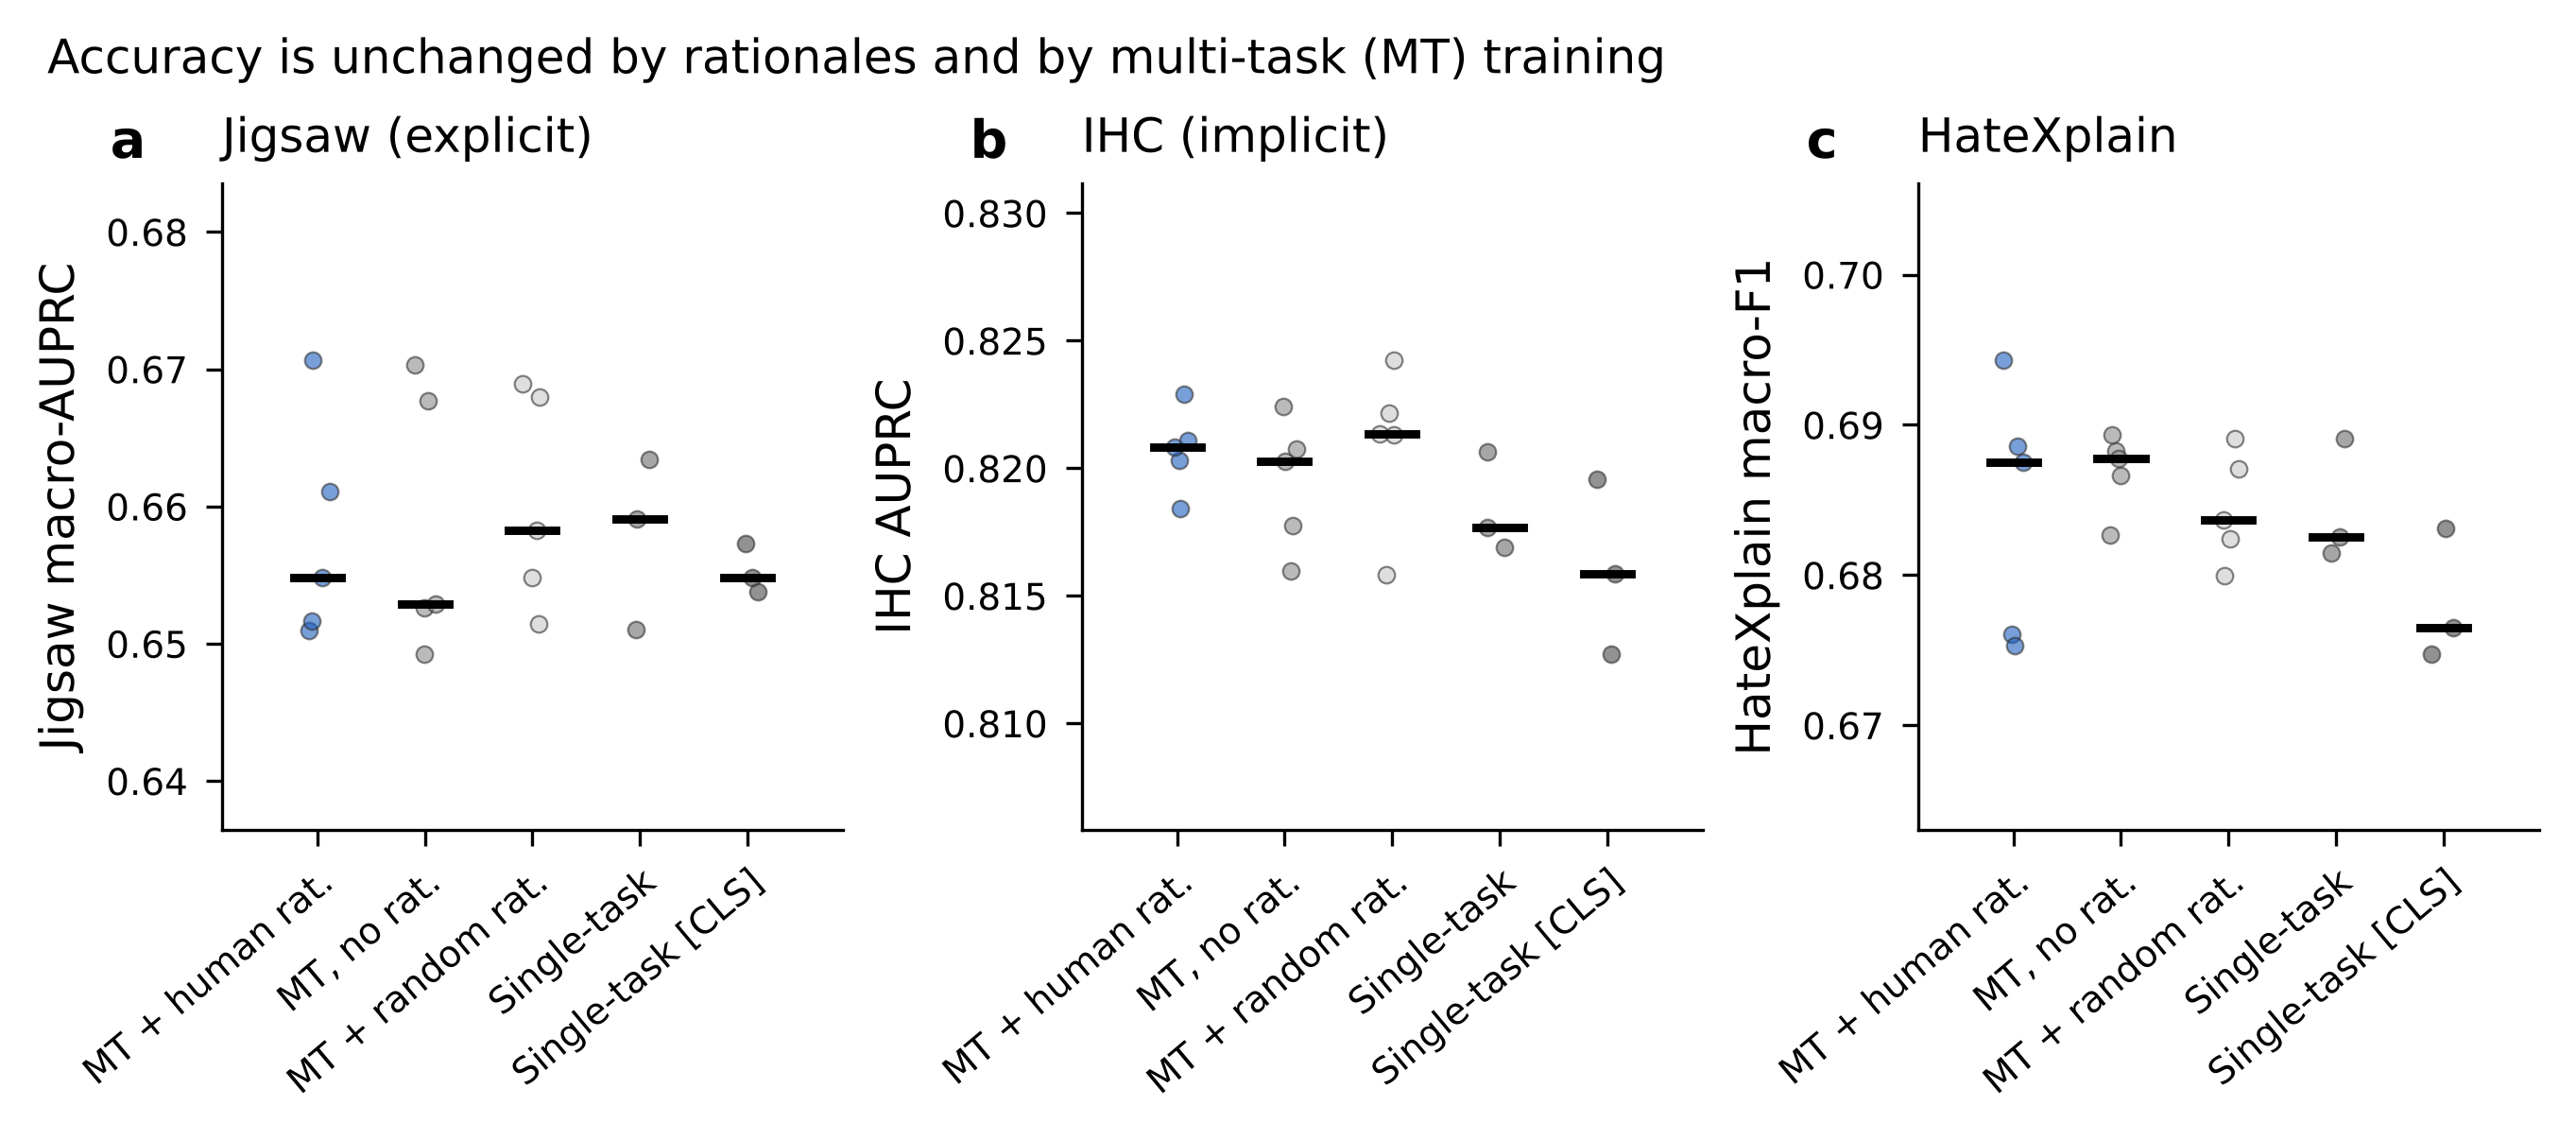
\includegraphics[width=\textwidth]{figures/fig_classification_parity.png}
\caption{Classification scores per seed on the three test sets. Rationale supervision (M1) and the controls (M2, M3) are indistinguishable from each other and from single-task models.}
\label{fig:parity}
\end{figure}

\subsection{Plausibility and faithfulness of the attention}
Figure~\ref{fig:h2} shows the H2 results. Without rationale supervision (M2), the HateXplain head's attention is already well above random on plausibility (0.688 vs.\ 0.381), and human rationales raise it to 0.924. Supervising with random-matched targets (M3) drives plausibility close to random (0.398) and destroys faithfulness (0.012), which confirms that the loss controls what the attention points to and that the gain of M1 comes from the human rationales themselves. Faithfulness and plausibility rise together: the words that humans mark are also the words whose deletion changes the model's prediction most. Sufficiency moves in the same direction ($-0.522$ for M1 vs.\ $-0.318$ for M2, lower is better). The gain does not depend on multi-task training: the single-task M6 reaches the same plausibility as M1 (0.924; +0.254 over M5, exploratory), and a shared attention pool (M4) gives the same plausibility as per-task pools.

\begin{figure}[t]
\centering
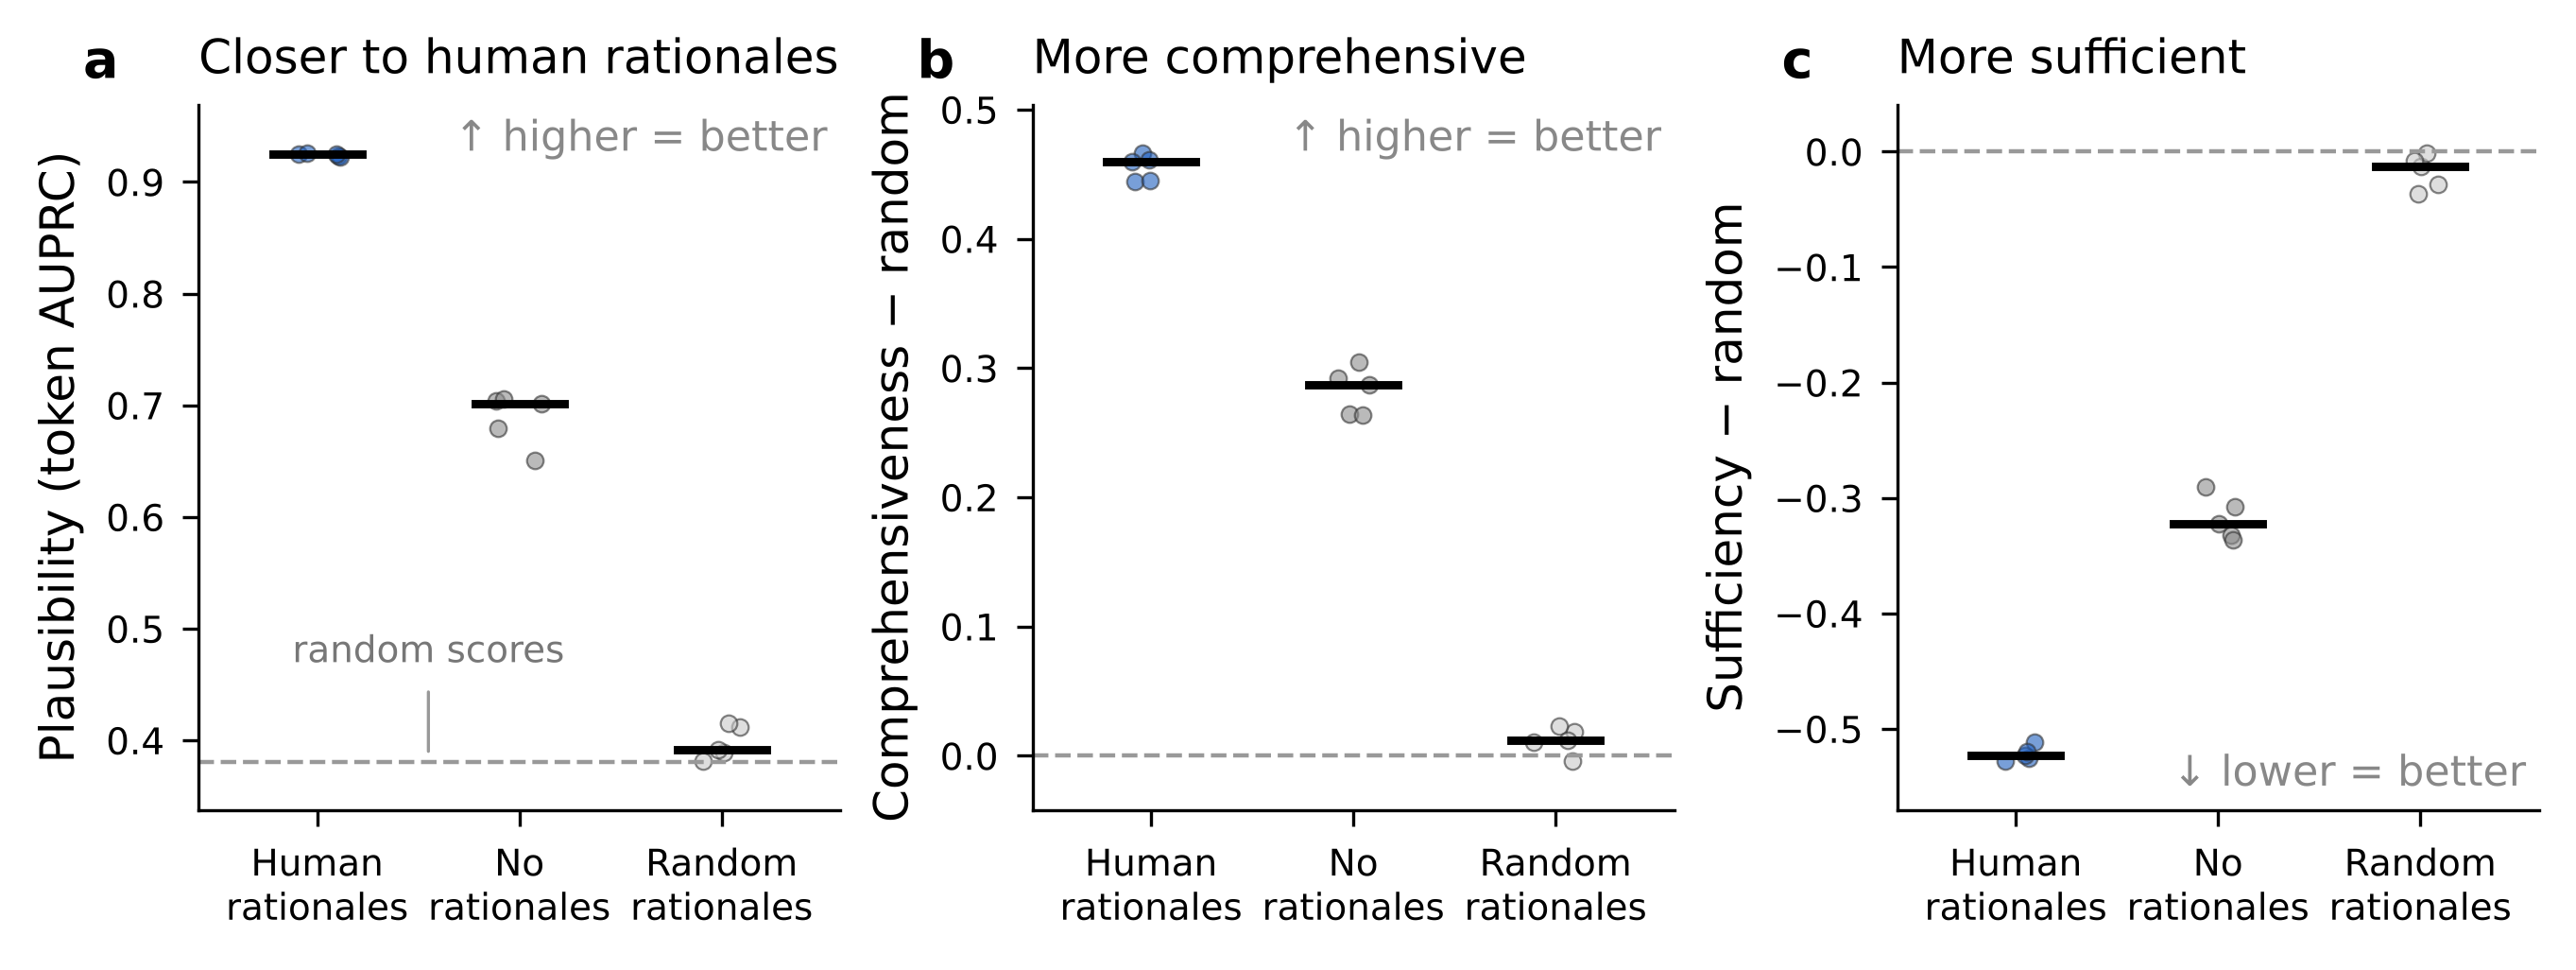
\includegraphics[width=\textwidth]{figures/fig_h2_explanations.png}
\caption{Plausibility (token-AUPRC) and faithfulness (AOPC comprehensiveness minus random) of the HateXplain head's attention, per seed. The dashed line marks random word scores.}
\label{fig:h2}
\end{figure}

\subsection{Transfer to heads without rationales}
The explicit-toxicity head never receives rationale supervision, yet under M1 its attention reaches a plausibility of 0.894 on HateXplain posts, against at most 0.551 under M2 and M3 (Figure~\ref{fig:h3}). Its faithfulness also rises (comprehensiveness minus random 0.326 vs.\ 0.082 under M2; exploratory, $p<10^{-8}$). The implicit-hate head gains less: plausibility 0.608 vs.\ 0.542 (not significant) and comprehensiveness 0.166 vs.\ 0.113 (exploratory, $p=0.005$). Because the heads have separate pools, the transfer must run through the shared encoder: rationale supervision changes the representations so that every pool finds the abusive words more easily. That the effect is weaker for implicit hate is consistent with implicit hate being carried less by individual words.

\begin{figure}[t]
\centering
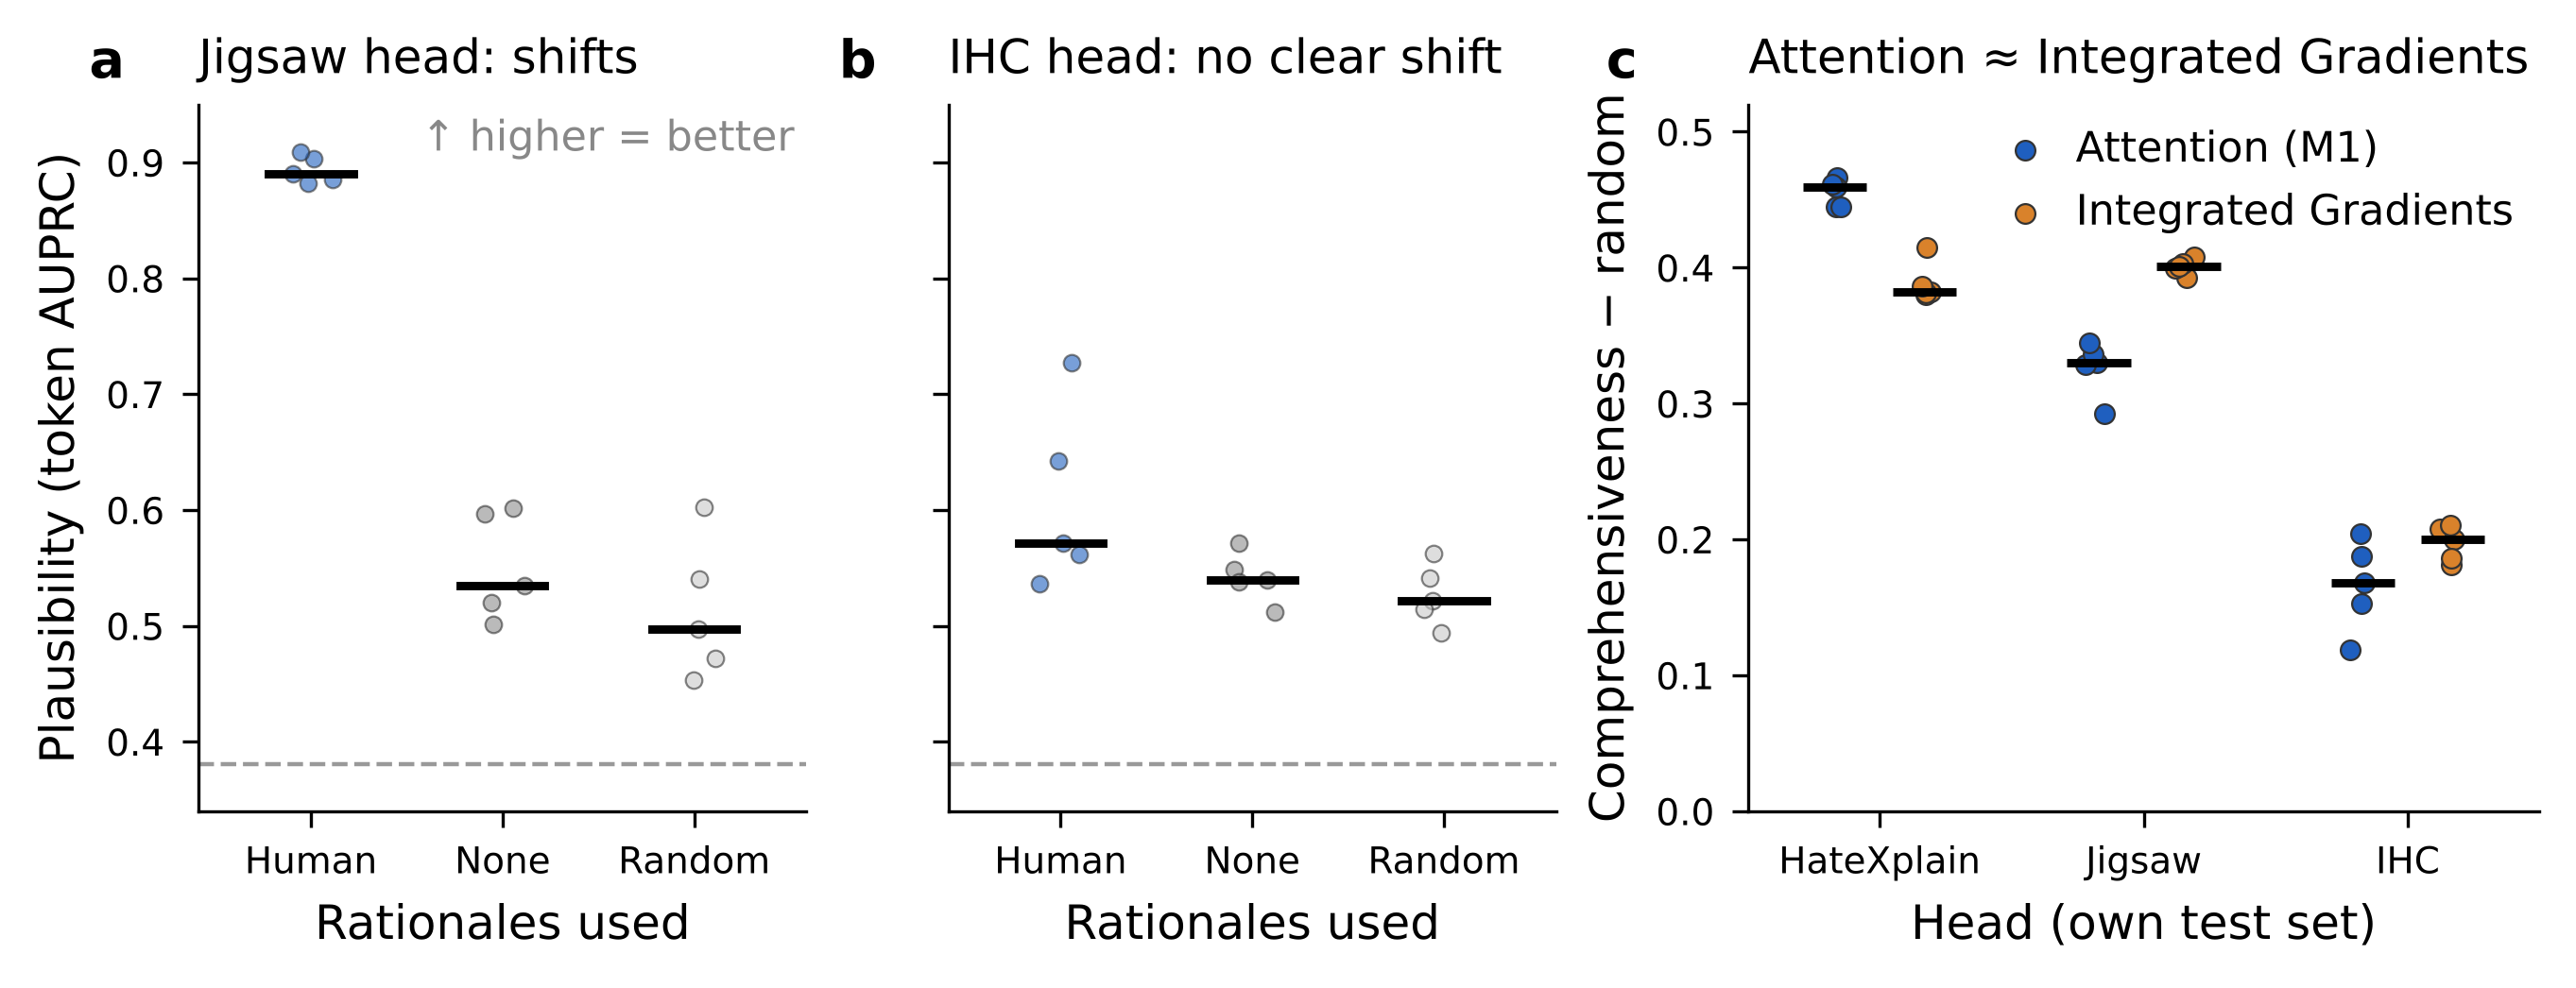
\includegraphics[width=\textwidth]{figures/fig_h3_transfer_and_ig.png}
\caption{Left: plausibility of each head's attention on HateXplain posts. Right: faithfulness of M1's attention against Integrated Gradients on each head's fixed post set.}
\label{fig:h3}
\end{figure}

\subsection{Attention versus post-hoc explainers}
Table~\ref{tab:efficiency} compares M1's attention with IG on the same posts. On the HateXplain head the attention is \emph{more} faithful than IG (0.455 vs.\ 0.389 comprehensiveness minus random; difference 0.066, 95\% CI [0.047, 0.086]). On the explicit and implicit heads IG is somewhat more faithful (differences $-0.075$ and $-0.031$), but both gaps are well inside the non-inferiority margins ($\delta=0.149$ and $0.081$), so E4 passes for all heads. E5 also passes: M1's attention is more faithful than M2's on every head.

Extracting the attention costs nothing measurable (Table~\ref{tab:efficiency}, Figure~\ref{fig:latency}). On a T4 GPU, prediction alone takes 15.4\,ms per post and prediction plus attention 15.2\,ms (ratio 0.99; E1 passes), with a 95th-percentile latency of 18.6\,ms (E3 passes). IG takes 72.4\,ms and LIME 346.6\,ms, 4.8$\times$ and 22.8$\times$ prediction plus attention, so E2 fails on GPU for both explainers. On a 4-thread CPU the picture changes: prediction plus attention takes 81\,ms (95th percentile 143\,ms; E3 passes), IG 4.2\,s and LIME 22.8\,s, 52$\times$ and 281$\times$ as long, so E1 and E2 pass on CPU. Prediction plus attention was measured as slightly faster than prediction alone on CPU (ratio 0.86); both run the same forward pass, so this reflects timing noise on a shared machine, and we read it as no difference. Because the criteria required E2 to hold on both devices, the efficiency claim E is not accepted as a whole. The GPU is so fast at the backward passes IG needs that the gap there is small; on CPU, where many moderation services run, the attention explanation is one to two orders of magnitude cheaper.

\begin{table}[t]
\centering
\caption{Efficiency criteria for M1. Timing at batch size 1: GPU, NVIDIA T4, three seeds; CPU, 4 threads, one seed. Faithfulness criteria use five seeds.}
\label{tab:efficiency}
\small
\resizebox{\textwidth}{!}{\begin{tabular}{llccc}
\toprule
Criterion & Measure & GPU & CPU & Pass \\
\midrule
E1 & time(pred.+attention) / time(pred.), target $\le1.05$ & 0.99 & 0.86 & yes / yes \\
E2 & IG time / pred.+attention, target $\ge10\times$ & 4.8$\times$ & 52.2$\times$ & no / yes \\
   & LIME time / pred.+attention, target $\ge100\times$ & 22.8$\times$ & 280.5$\times$ & no / yes \\
E3 & 95th-percentile latency of pred.+attention & 18.6\,ms ($<100$) & 143\,ms ($<1000$) & yes / yes \\
E4 & comp.\ attention $-$ IG: HX / Jigsaw / IHC head & \multicolumn{2}{c}{0.066 / $-0.075$ / $-0.031$} & yes (all heads) \\
E5 & comp.\ M1 $-$ M2 attention: HX / Jigsaw / IHC & \multicolumn{2}{c}{0.173 / 0.244 / 0.053} & yes (all heads) \\
\bottomrule
\end{tabular}}
\end{table}

\begin{figure}[t]
\centering
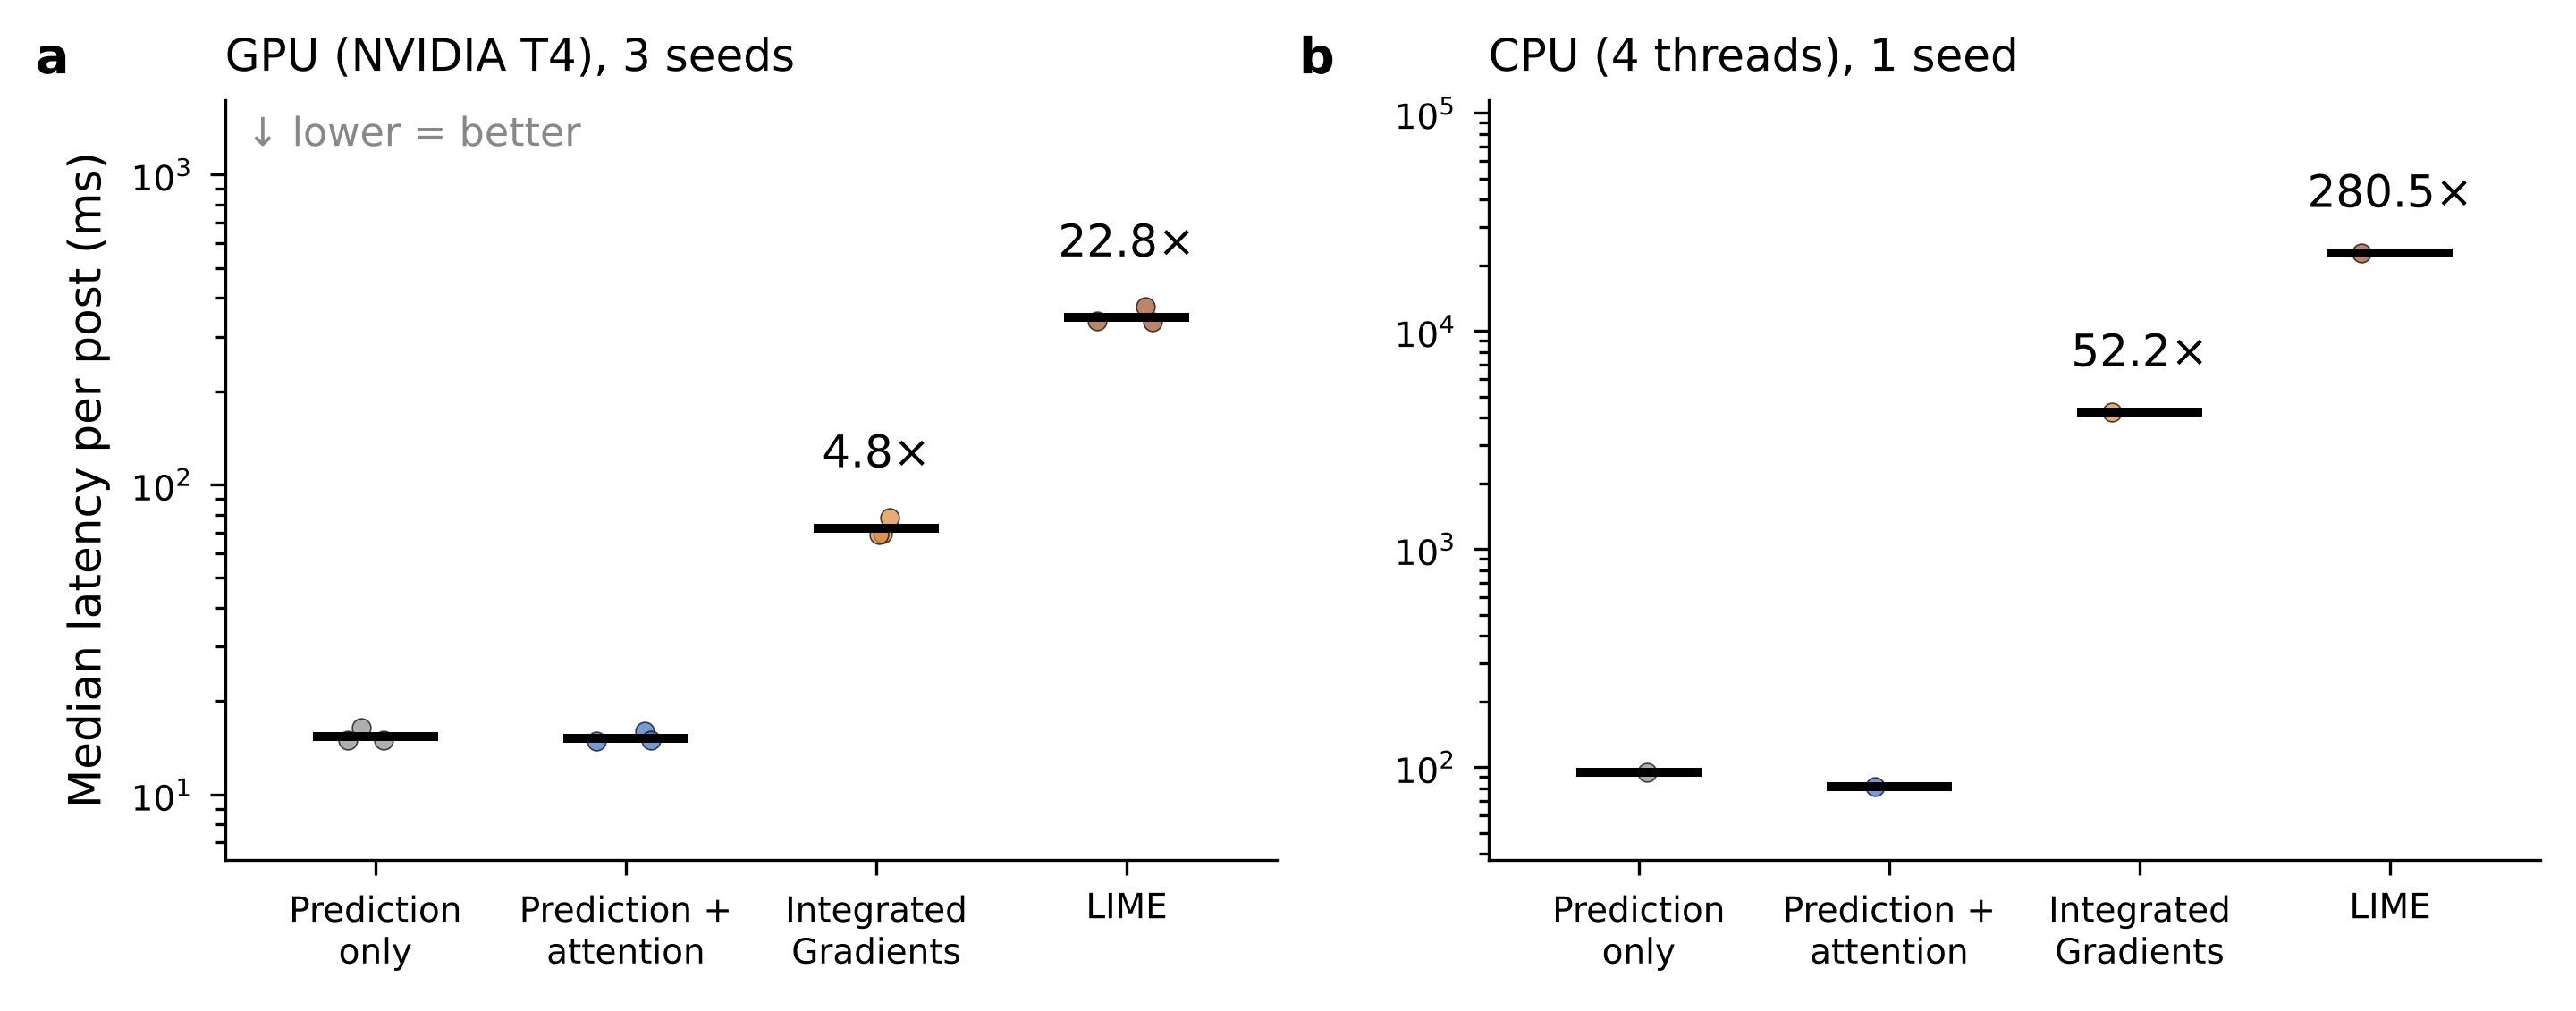
\includegraphics[width=\textwidth]{figures/fig_latency_gpu_cpu.png}
\caption{Per-post latency of RAMT (M1) at batch size 1 (log scale). (a) NVIDIA T4 GPU, three seeds; (b) 4-thread CPU, one seed. Black lines: median over all posts pooled across seeds; dots: per-seed medians. Labels give IG and LIME latency as multiples of prediction plus attention.}
\label{fig:latency}
\end{figure}

\subsection{Bias and functional tests}
\label{sec:bias}
Every rationale-trained model has a lower GMB-BPSN than its counterpart without rationales (HateXplain protocol, Table~\ref{tab:hxprotocol}): M1 0.708 vs.\ M2 0.744, M4 0.713 vs.\ M4b 0.740, M6 0.714 vs.\ M5 0.746. The confirmatory test is not significant ($p=0.654$), because per-community BPSN on the 1{,}924 test posts is noisy (test-sampling variance 0.0060 against seed variance 0.0003), but M1 is lower than M2 in all five seeds. The gap comes mainly from two small communities, Hispanic (BPSN 0.54 vs.\ 0.61) and Arab (0.64 vs.\ 0.68); the other eight differ by at most 0.01. A plausible reading is that rationales often mark identity terms, so rationale-trained attention leans on them and confuses benign posts that mention a group with hateful ones. On HateCheck, the share of non-hateful cases flagged by the HateXplain head is about 0.6 for the multi-task models and about 0.33 for single-task models, with M1 slightly lower than M2 and M3 (exploratory, not significant).

%% ===================================================================
\section{Discussion and limitations}
\label{sec:discussion}

\paragraph{What rationale supervision buys}
For a moderation tool the main result is practical: one extra loss term, at no measurable cost in accuracy, makes the model's own attention a plausible and faithful explanation that is available at prediction time. On the task it was trained on, that attention is more faithful than IG. The random-matched control shows that this is not a side effect of constraining attention: the same constraint on the wrong words produces explanations that are neither plausible nor faithful.

\paragraph{Use in a moderation pipeline}
In deployment, one encoder pass serves all three heads, and each head's attention gives a word-level highlight at no extra cost. A moderation queue can therefore show the flagged post with its highlighted words immediately, and reserve slower post-hoc explainers such as IG for appeals or audits. Because the HateXplain head's attention is more faithful than IG on its own task, the highlight shown to the moderator is also the better guide to what the model actually used.

\paragraph{Multi-task training}
H1 failed. Sharing an encoder across Jigsaw, IHC and HateXplain neither helped nor hurt, so multi-task training is justified here by deployment (one encoder pass serves three heads) and by the transfer of explanation quality, not by accuracy.

\paragraph{Limitations}
\begin{itemize}
\item \textbf{Speed target.} E2 failed on GPU: IG was only 4.8$\times$ and LIME 22.8$\times$ slower than prediction plus attention, below the targets set in advance (10$\times$ and 100$\times$), although both targets were met on CPU. The absolute saving on GPU (57\,ms per post against IG) may still matter at scale, but the claim as specified is not supported.
\item \textbf{IG completeness.} With 50 steps, the IG completeness gap exceeded 5\% of the output on 20\%, 25\% and 36\% of posts for the HateXplain, Jigsaw and IHC heads (medians 1.1--2.5\%). IG with more steps might be somewhat more faithful, so E4 should be read with this in mind.
\item \textbf{Bias.} Rationale-trained models score consistently, though not significantly, lower on GMB-BPSN. The test is underpowered, and the gap is concentrated in two small communities; a larger targeted evaluation is needed before deployment.
\item \textbf{Plausibility ceiling.} Leave-one-annotator-out agreement (0.689) is lower than M1's plausibility (0.924) because a single annotator's binary marks are heavily tied scores; it is therefore an inter-annotator reference, not a ceiling, and we report raw plausibility with the random floor.
\item \textbf{Units.} We evaluate explanations over words; HateXplain's published numbers use BERT word pieces, so absolute values are not directly comparable. A reimplementation of HateXplain's protocol is in \ref{app:hatexplain}; it gives the same conclusions.
\item \textbf{CPU timing} was measured with one seed because three seeds exceeded the 12-hour compute limit; GPU medians of the three seeds agreed within 10\%, and the CPU ratios (52$\times$, 281$\times$) are far from the thresholds. Timings on shared cloud machines are noisy, as the CPU ratio of 0.86 for E1 shows.
\item \textbf{Scope.} English only; one encoder size; rationales from one dataset.
\end{itemize}

%% ===================================================================
\section{Conclusion}
\label{sec:conclusion}
Supervising the attention of one head of a multi-task hate-speech detector with human rationales made its attention markedly more plausible and more faithful, without changing classification, and the improvement carried over to a head that never saw rationales. On its own task the supervised attention was more faithful than Integrated Gradients and cost nothing extra at inference. Multi-task training brought no accuracy gain, the speed targets set in advance were met on CPU but missed on GPU, and a consistent, non-significant drop in a subgroup-bias metric calls for a targeted fairness evaluation before deployment.

\section*{Data availability}
HateXplain is available under the MIT licence. The Implicit Hate Corpus is used under CC BY 4.0 with attribution to \citet{elsherief2021latent}; tweet text is not redistributed. HateCheck is available under CC BY 4.0. The Jigsaw data are used under the Kaggle competition rules. \todo{OLID licence if OLID is used; repository link for code and split identifiers.}

\section*{CRediT authorship contribution statement}
\textbf{Veena Shanmukh Bagildavar:} \todo{contributions}
\textbf{Varsha Shivanand K:} \todo{contributions}
\textbf{Yashwitha T S:} \todo{contributions}
\textbf{Madderla Chiranjeevi:} \todo{e.g.\ Supervision, Conceptualization, Writing -- review \& editing.}

\section*{Declaration of competing interest}
\todo{The authors declare that they have no known competing financial interests or personal relationships that could have appeared to influence the work reported in this paper.}

\section*{Declaration of generative AI use}
\todo{EAAI requires a statement on the use of generative AI in writing; please complete it.}

\appendix
\section{HateXplain protocol}
\label{app:hatexplain}
To ease comparison with the HateXplain paper, Table~\ref{tab:hxprotocol} re-scores the HateXplain head with HateXplain's own evaluation protocol, which we reimplemented from the authors' code and checked against ERASER's reference implementation on 300 random posts (differences below $10^{-9}$). Classification: accuracy, macro-F1 and one-vs-one macro AUROC on the 1{,}924 test posts. Plausibility: on the 1{,}142 hateful or offensive test posts, the gold rationale is the union of the annotators' marks and the model rationale is the top five words by attention; IOU-F1 (threshold 0.5) and token-F1 follow ERASER, and AUPRC uses the attention scores directly. Bias: the generalised-mean Subgroup, BPSN and BNSP AUCs ($p=-5$) over the ten most-targeted communities, excluding posts that target none of them. Our explanations are scored over words, whereas HateXplain scores BERT word pieces, so absolute plausibility values are not directly comparable with the published ones.

\begin{table}[h]
\centering
\caption{HateXplain head under HateXplain's protocol, mean $\pm$ s.d.\ over seeds (5 for M1--M3, 3 otherwise). Higher is better for all columns.}
\label{tab:hxprotocol}
\resizebox{\textwidth}{!}{\begin{tabular}{lccccccccc}
\toprule
Model & Accuracy & Macro-F1 & AUROC & IOU-F1 & Token-F1 & AUPRC & GMB-Sub. & GMB-BPSN & GMB-BNSP \\
\midrule
M1 RAMT & 0.699$\pm$0.006 & 0.684$\pm$0.008 & 0.859$\pm$0.002 & 0.375$\pm$0.002 & 0.548$\pm$0.002 & 0.915$\pm$0.001 & 0.796$\pm$0.016 & 0.708$\pm$0.022 & 0.805$\pm$0.009 \\
M2 & 0.702$\pm$0.005 & 0.687$\pm$0.003 & 0.859$\pm$0.002 & 0.286$\pm$0.013 & 0.446$\pm$0.014 & 0.681$\pm$0.020 & 0.812$\pm$0.008 & 0.744$\pm$0.030 & 0.803$\pm$0.009 \\
M3 & 0.700$\pm$0.002 & 0.684$\pm$0.004 & 0.858$\pm$0.002 & 0.137$\pm$0.008 & 0.283$\pm$0.011 & 0.452$\pm$0.010 & 0.807$\pm$0.008 & 0.751$\pm$0.025 & 0.796$\pm$0.008 \\
M4 & 0.695$\pm$0.006 & 0.681$\pm$0.007 & 0.858$\pm$0.002 & 0.373$\pm$0.003 & 0.547$\pm$0.000 & 0.915$\pm$0.001 & 0.801$\pm$0.008 & 0.713$\pm$0.017 & 0.794$\pm$0.013 \\
M4b & 0.698$\pm$0.005 & 0.683$\pm$0.003 & 0.858$\pm$0.002 & 0.228$\pm$0.003 & 0.366$\pm$0.004 & 0.567$\pm$0.006 & 0.807$\pm$0.009 & 0.740$\pm$0.021 & 0.795$\pm$0.004 \\
M5 (HX only) & 0.696$\pm$0.006 & 0.684$\pm$0.004 & 0.859$\pm$0.001 & 0.283$\pm$0.025 & 0.436$\pm$0.033 & 0.665$\pm$0.052 & 0.800$\pm$0.008 & 0.746$\pm$0.012 & 0.792$\pm$0.021 \\
M6 (HX + rationale) & 0.693$\pm$0.010 & 0.682$\pm$0.007 & 0.855$\pm$0.006 & 0.378$\pm$0.004 & 0.550$\pm$0.004 & 0.916$\pm$0.005 & 0.775$\pm$0.037 & 0.714$\pm$0.033 & 0.800$\pm$0.009 \\
M8 HateBERT & 0.701$\pm$0.002 & 0.689$\pm$0.003 & 0.858$\pm$0.002 & 0.273$\pm$0.018 & 0.432$\pm$0.021 & 0.678$\pm$0.031 & 0.802$\pm$0.007 & 0.699$\pm$0.028 & 0.804$\pm$0.003 \\
M8 DeBERTa-v3 & 0.702$\pm$0.009 & 0.689$\pm$0.011 & 0.862$\pm$0.005 & 0.263$\pm$0.024 & 0.411$\pm$0.033 & 0.616$\pm$0.043 & 0.823$\pm$0.004 & 0.753$\pm$0.004 & 0.814$\pm$0.002 \\
CLS (HX only) & 0.690$\pm$0.002 & 0.678$\pm$0.004 & 0.855$\pm$0.002 & -- & -- & -- & 0.809$\pm$0.012 & 0.751$\pm$0.004 & 0.795$\pm$0.009 \\
\bottomrule
\end{tabular}}
\end{table}

Faithfulness under the same protocol (one-shot deletion or retention of the top-five words; comprehensiveness higher and sufficiency lower is better) gives the same ranking as the AOPC measure in the main text: M1 comprehensiveness $0.585\pm0.012$ and sufficiency $0.040\pm0.007$; M2 $0.488\pm0.019$ and $0.110\pm0.015$; M3 $0.183\pm0.014$ and $0.400\pm0.020$ (five seeds each).

\section{Shortcut check on the Implicit Hate Corpus}
\label{app:ihc}
Because IHC posts are tweets, labels could correlate with surface features such as retweet markers, quotes, mentions, URLs, hashtags or length. A logistic regression on these seven features alone reaches a test AUROC of only 0.562, against 0.82 for our models, so the IHC results are not explained by such shortcuts.

\bibliographystyle{elsarticle-harv}
\bibliography{references}

\end{document}
